\documentclass{beamer}
\usetheme{Boadilla}
\usepackage{siunitx}
\usepackage{amsmath}
\usepackage{graphicx}
\usepackage[labelformat=empty]{caption}
\usepackage{verbatim}

\title[Bioprocessing facilities design]{Dissertation:
    Optimising the design of buffer preparation in bioprocessing facilities}
\subtitle{MSc in Business Analytics (Part Time) 2015--2017}
\author{Sean Tully}
\institute{University College Dublin}
\date{25\textsuperscript{th} August 2017}

\begin{document}
\setbeamertemplate{caption}{\raggedright\insertcaption\par}

\begin{frame}
    \titlepage
\end{frame}


\begin{frame}
    \frametitle{Introduction -- Problem Definition}
    \begin{columns}
        \column{0.65\textwidth}
            \begin{itemize}
                \item Bioprocessing involves the synthesis of therapeutic
                    products using biological agents (bacteria or mammalian
                    cells)        
                \item The purification of these products typically requires the
                    use of 10--20 different buffer solutions (\emph{buffers})
                \item Calculating the correct number and volume of vessels for
                    buffer preparation in a large-scale facility represents a
                    significant engineering challenge
                \item The aim of this work was to develop a methodology for
                    calculating buffer vessel requirements, given some process
                    information
            \end{itemize}        
        \column{0.35\textwidth}
        \begin{figure}
            \centering
            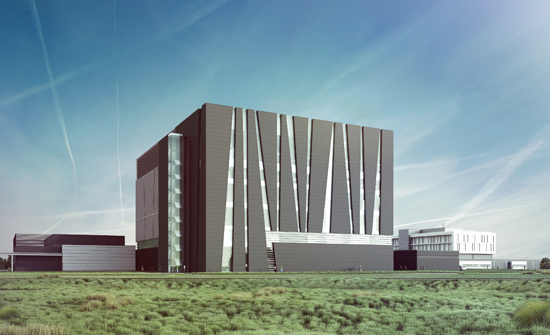
\includegraphics[width=0.95\textwidth]{alexion.jpg}\\
            \vspace{0.3cm}
            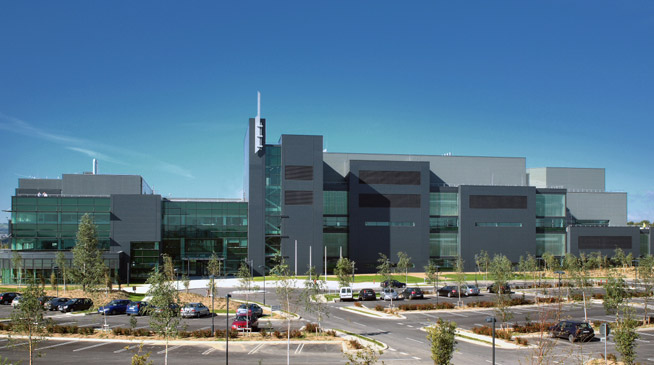
\includegraphics[width=0.95\textwidth]{janssen.jpg}
            \caption{\scriptsize Top: Alexion, Dublin. Bottom:
                Janssen Biologics, Cork (formerly Centocor).
                Both images \copyright PM~Group.}
        \end{figure}
    \end{columns}
\end{frame}

\begin{frame}
    \frametitle{Buffer Preparation}
    \begin{columns}
        \column{0.5\textwidth}
        \begin{itemize}
            \item Buffer preparation requires two vessels
            \item Each buffer is prepared in a \emph{preparation vessel}, which
                may be used to prepare many buffers
            \item It is assumed that each buffer has a dedicated \emph{hold
                vessel}
            \item We want to minimise the total cost of vessels in buffer
                preparation.
        \end{itemize}
        \column{0.5\textwidth}
        \begin{figure}
            \centering
            \includegraphics[angle=0,scale=0.5]{./../figures/buffer_pfd.pdf}
            \caption{\scriptsize Single buffer preparation -- equipment}
        \end{figure}
    \end{columns}
\end{frame}

\begin{frame}
    \frametitle{Existing Workflow}
    \begin{itemize}
        \item Model production schedule using a software package such as
        SchedulePro
        \item Run the model with a dedicated preparation vessel for every hold
        vessel
        \item Remove preparation vessels until no more can be removed
        \begin{itemize}
            \item \emph{involves trial and error}
        \end{itemize}
        \item Stop when you can't find a way to remove any more vessels
        \begin{itemize}
            \item \emph{no guarantee that the optimum selection has been found}
        \end{itemize}
    \end{itemize}
    \begin{figure}
        \centering
        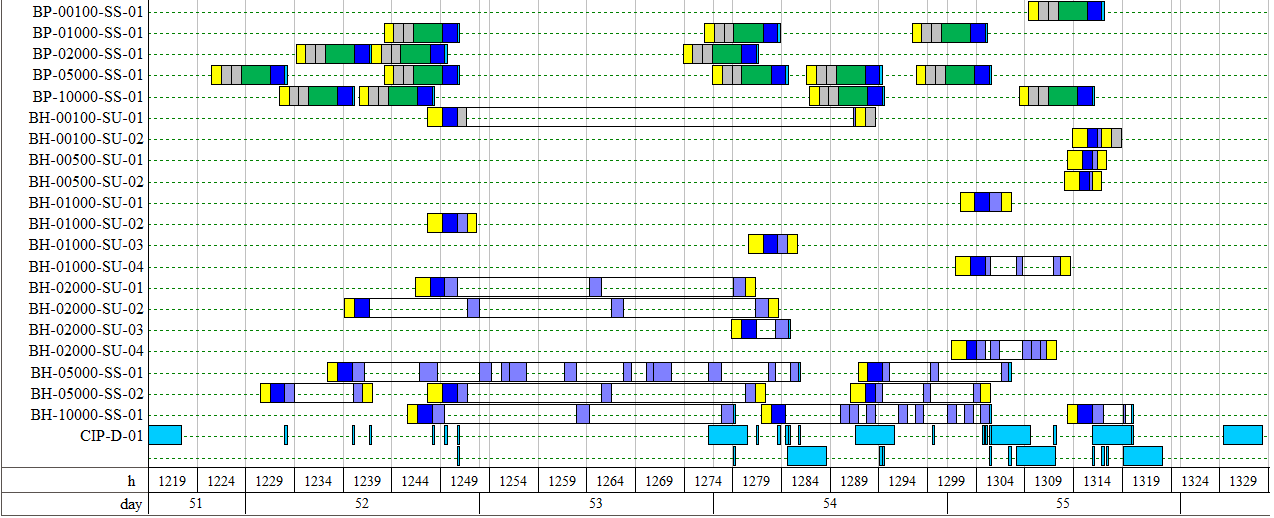
\includegraphics[angle=0,scale=0.2]{schedulepro.png}
    \end{figure}
\end{frame}

\begin{frame}
    \frametitle{Proposition}
    \begin{itemize}
    \item Find optimum vessel selection to minimise cost, using Mixed Integer
    Linear Programming (MILP)
    \end{itemize}
\end{frame}

\begin{comment}
\begin{frame}
    \frametitle{Buffer Preparation Scheduling}
    \begin{figure}
        \centering
        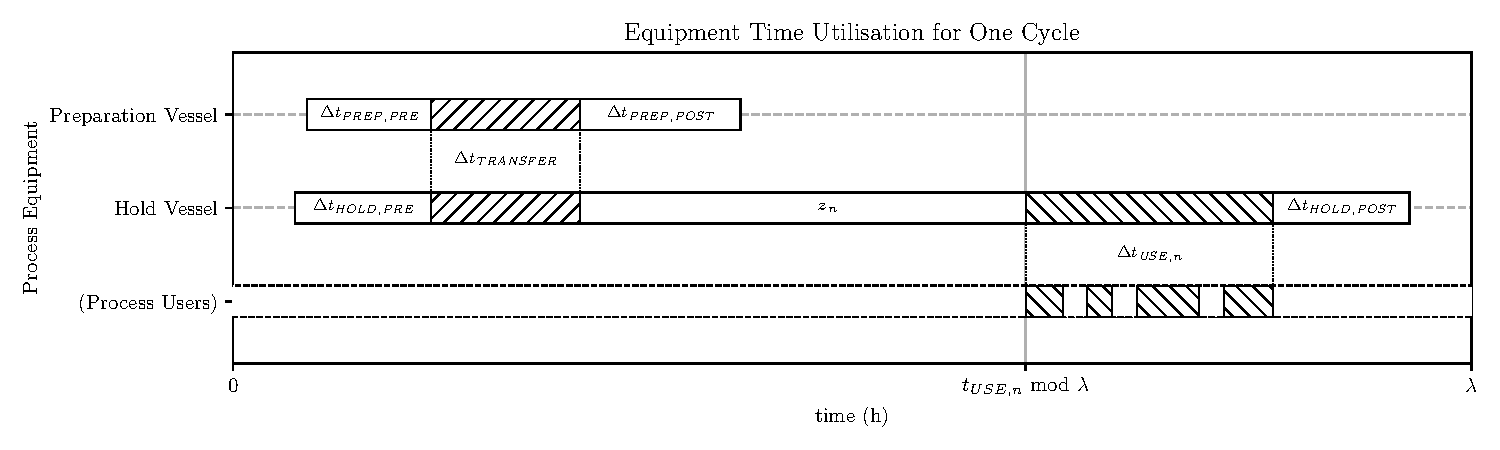
\includegraphics[angle=0,scale=0.45]{./../figures/explanatory.pdf}
        \caption{\scriptsize Single buffer preparation -- scheduling}
    \end{figure}
    \begin{itemize}
    \item The volume of each buffer is known, as is it's time of first use and
        total duration of use
    \item Some flexibility exists in the hold duration and in vessel selection
    \end{itemize}
\end{frame}
\end{comment}

\begin{frame}
    \frametitle{Input Data}
    \begin{columns}
        \column{0.65\textwidth}
        \centering \small Buffer Data\\
            \begin{table}
            \scriptsize
                \begin{tabular}{l | r | r | r}
                    names & volumes & use start times & use durations\\
                    & $U_{n}$ (l) & $t_{\mathit{USE},n}^{*}$ (h) 
                    & $\Delta t_{\mathit{USE},n}$
                    (h)\\ \hline
                    \text{Buffer \#1} & \SI{24427.13}{} & \SI{76.23}{}
                    & \SI{20.56}{}\\
                    \text{Buffer \#2} & \SI{5487.29}{} & \SI{0.21}{}
                    & \SI{49.77}{}\\
                    \text{Buffer \#3} & \SI{2588.36}{} & \SI{25.78}{}
                    & \SI{24.56}{}\\
                    \text{Buffer \#4} & \SI{7102.05}{} & \SI{46.79}{}
                    & \SI{27.77}{}\\
                    \text{Buffer \#5} & \SI{1020.87}{} & \SI{87.70}{}
                    & \SI{36.58}{}\\
                    \text{Buffer \#6} & \SI{19508.79}{} & \SI{35.52}{}
                    & \SI{58.53}{}\\
                    \text{Buffer \#7} & \SI{23073.55}{} & \SI{42.26}{}
                    & \SI{39.71}{}\\
                    \text{Buffer \#8} & \SI{25454.10}{} & \SI{48.38}{}
                    & \SI{43.47}{}\\
                    \text{Buffer \#9} & \SI{24088.67}{} & \SI{4.18}{}
                    & \SI{55.41}{}\\
                    \text{Buffer \#10} & \SI{3172.46}{} & \SI{48.31}{}
                    & \SI{23.27}{}\\
                    \text{Buffer \#11} & \SI{24752.71}{} & \SI{76.38}{}
                    & \SI{45.80}{}\\
                    \text{Buffer \#12} & \SI{13445.31}{} & \SI{73.93}{}
                    & \SI{34.25}{}\\
                \end{tabular}
            \end{table}
        \column{0.35\textwidth}
            \centering \small Vessel Data\\
            \begin{table}
                \scriptsize
                \begin{tabular}{l | r | r}
                    names & volumes & costs\\
                    & $V_{m}$ (l) & $c_{m}$ (--)\\\hline
                    \SI{1000}{\litre} & \SI{1000.0}{} & \SI{63.10}{}\\
                    \SI{2000}{\litre} & \SI{2000.0}{} & \SI{95.64}{}\\
                    \SI{3000}{\litre} & \SI{3000.0}{} & \SI{121.98}{}\\
                    \SI{4000}{\litre} & \SI{4000.0}{} & \SI{144.96}{}\\
                    \SI{5000}{\litre} & \SI{5000.0}{} & \SI{165.72}{}\\
                    \SI{6000}{\litre} & \SI{6000.0}{} & \SI{184.88}{}\\
                    %\SI{8000}{\litre} & \SI{8000.0}{} & \SI{219.71}{}\\
                    %\SI{10000}{\litre} & \SI{10000.0}{} & \SI{251.19}{}\\
                    %\SI{12000}{\litre} & \SI{12000.0}{} & \SI{280.83}{}\\
                    %\SI{16000}{\litre} & \SI{16000.0}{} & \SI{333.02}{}\\
                    %\SI{18000}{\litre} & \SI{18000.0}{} & \SI{357.41}{}\\
                    \quad $\vdots$ & $\vdots\quad$ & $\vdots\quad$\\
                    \SI{20000}{\litre} & \SI{20000.0}{} & \SI{380.73}{}\\
                    \SI{22000}{\litre} & \SI{22000.0}{} & \SI{403.14}{}\\
                    \SI{25000}{\litre} & \SI{25000.0}{} & \SI{435.28}{}\\
                    \SI{30000}{\litre} & \SI{30000.0}{} & \SI{485.59}{}\\
                \end{tabular}
            \end{table}
    \end{columns}
\end{frame}

\begin{frame}
    \frametitle{Buffer Preparation Scheduling}
    \begin{figure}
        \centering
        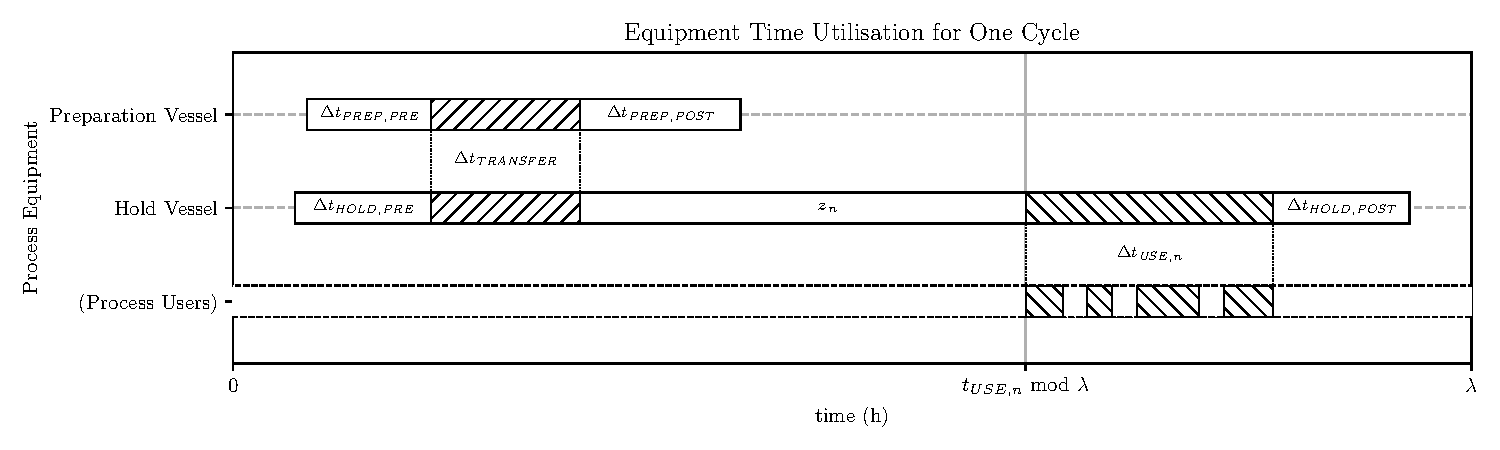
\includegraphics[width=\textwidth]{./../figures/explanatory.pdf}
    \end{figure}
    \begin{columns}
        \small
        \column{0.45\textwidth}
            \begin{itemize}
            \item The volume of each buffer is known, as is it's time of first
                use and total duration of use
            \item Some flexibility exists in the hold duration and in vessel
                selection
            \end{itemize}
        \column{0.55\textwidth}
            \centering \small Parameters\\
            \vspace{0.2cm}
            \tiny
            \begin{tabular}{l | l | r | c}
                symbol & short description & value & unit\\ \hline
                $T$ & process cycle time & 96.0 & h\\
                $\Delta t_{\mathit{PREP,PRE}}$ & prep pre duration & 12.0 & h\\
                $\Delta t_{\mathit{PREP,POST}}$ & prep post duration & 1.5 & h\\
                $\Delta t_{\mathit{TRANSFER}}$ & transfer duration & 2.0 & h\\
                $\Delta t_{\mathit{HOLD,PRE}}$ & hold pre duration & 8.0 & h\\
                $\Delta t_{\mathit{HOLD,POST}}$ & hold post duration & 1.5 & h\\
                $\Delta t_{\mathit{HOLD,MIN}}$ & minimum hold duration & 12.0 & h\\
                $\Delta t_{\mathit{HOLD,MAX}}$ & maximum hold duration & 60.0 & h\\
                $f_{\mathit{MINFILL}}$ & minimum fill ratio & 0.3 & --\\
                $f_{\mathit{UTIL}}$ & maximum utilisation ratio & 0.8 & --\\
            \end{tabular}
    \end{columns}
\end{frame}

\begin{comment}
\begin{frame}
    \frametitle{Global parameters for random example}
    \begin{table}
        \begin{tabular}{l | l | r | c}
            symbol & short description & value & unit\\ \hline
            $T$ & process cycle time & 96.0 & h\\
            $\Delta t_{\mathit{PREP,PRE}}$ & prep pre duration & 12.0 & h\\
            $\Delta t_{\mathit{PREP,POST}}$ & prep post duration & 1.5 & h\\
            $\Delta t_{\mathit{TRANSFER}}$ & transfer duration & 2.0 & h\\
            $\Delta t_{\mathit{HOLD,PRE}}$ & hold pre duration & 8.0 & h\\
            $\Delta t_{\mathit{HOLD,POST}}$ & hold post duration & 1.5 & h\\
            $\Delta t_{\mathit{HOLD,MIN}}$ & minimum hold duration & 12.0 & h\\
            $\Delta t_{\mathit{HOLD,MAX}}$ & maximum hold duration & 60.0 & h\\
            $f_{\mathit{MINFILL}}$ & minimum fill ratio & 0.3 & --\\
            $f_{\mathit{UTIL}}$ & maximum utilisation ratio & 0.8 & --\\
        \end{tabular}
    \end{table}
\end{frame}

\begin{frame}
    \frametitle{Vessel data for random example}
    \begin{table}
        \begin{tabular}{l | r | r}
            names & volumes & costs\\
            & $V_{m}$ (l) & $c_{m}$ (--)\\\hline
            \SI{1000}{\litre} & \SI{1000.0}{} & \SI{63.10}{}\\
            \SI{2000}{\litre} & \SI{2000.0}{} & \SI{95.64}{}\\
            \SI{3000}{\litre} & \SI{3000.0}{} & \SI{121.98}{}\\
            \SI{4000}{\litre} & \SI{4000.0}{} & \SI{144.96}{}\\
            %\SI{5000}{\litre} & \SI{5000.0}{} & \SI{165.72}{}\\
            %\SI{6000}{\litre} & \SI{6000.0}{} & \SI{184.88}{}\\
            %\SI{8000}{\litre} & \SI{8000.0}{} & \SI{219.71}{}\\
            %\SI{10000}{\litre} & \SI{10000.0}{} & \SI{251.19}{}\\
            %\SI{12000}{\litre} & \SI{12000.0}{} & \SI{280.83}{}\\
            %\SI{16000}{\litre} & \SI{16000.0}{} & \SI{333.02}{}\\
            %\SI{18000}{\litre} & \SI{18000.0}{} & \SI{357.41}{}\\
            $\quad\vdots$ & $\vdots\quad$ & $\vdots\quad$\\
            \SI{20000}{\litre} & \SI{20000.0}{} & \SI{380.73}{}\\
            \SI{22000}{\litre} & \SI{22000.0}{} & \SI{403.14}{}\\
            \SI{25000}{\litre} & \SI{25000.0}{} & \SI{435.28}{}\\
            \SI{30000}{\litre} & \SI{30000.0}{} & \SI{485.59}{}\\
        \end{tabular}
    \end{table}
\end{frame}

\begin{frame}
    \frametitle{Buffer data for random example}
    \begin{table}
        \centering
        \label{tbl.buffer}
        \begin{tabular}{l | c | c | c}
            names & required volumes & use start times & use durations\\
            & $U_{n}$ (l) & $t_{\mathit{USE},n}^{*}$ (h) 
            & $\Delta t_{\mathit{USE},n}$
            (h)\\ \hline
            \text{Buffer \#1} & \SI{24427.13}{} & \SI{76.23}{} & \SI{20.56}{}\\
            \text{Buffer \#2} & \SI{5487.29}{} & \SI{0.21}{} & \SI{49.77}{}\\
            \text{Buffer \#3} & \SI{2588.36}{} & \SI{25.78}{} & \SI{24.56}{}\\
            \text{Buffer \#4} & \SI{7102.05}{} & \SI{46.79}{} & \SI{27.77}{}\\
            \text{Buffer \#5} & \SI{1020.87}{} & \SI{87.7}{} & \SI{36.58}{}\\
            \text{Buffer \#6} & \SI{19508.79}{} & \SI{35.52}{} & \SI{58.53}{}\\
            \text{Buffer \#7} & \SI{23073.55}{} & \SI{42.26}{} & \SI{39.71}{}\\
            \text{Buffer \#8} & \SI{25454.10}{} & \SI{48.38}{} & \SI{43.47}{}\\
            \text{Buffer \#9} & \SI{24088.67}{} & \SI{4.18}{} & \SI{55.41}{}\\
            \text{Buffer \#10} & \SI{3172.46}{} & \SI{48.31}{} & \SI{23.27}{}\\
            \text{Buffer \#11} & \SI{24752.71}{} & \SI{76.38}{} & \SI{45.80}{}\\
            \text{Buffer \#12} & \SI{13445.31}{} & \SI{73.93}{} & \SI{34.25}{}\\
        \end{tabular}
    \end{table}
\end{frame}
\end{comment}

\begin{comment}
\begin{frame}
    \frametitle{Basic Model}
    Objective Function: Minimise total preparation vessel cost\\
    \begin{equation}
        \boldsymbol{Z} = \sum_{m \in \mathcal{M}} \sum_{p \in \mathcal{P}} c_m
        \boldsymbol{y}_{mp}
    \end{equation}
    Subject to \ldots
    \begin{itemize}
    \item Each buffer must be prepared in exactly one slot\\
    \begin{equation}
        \sum_{p \in \mathcal{P}} \boldsymbol{x}_{np} = 1 \quad \forall n \in 
        \mathcal{N}
    \end{equation}
    \item Each slot may contain at most one vessel instance
    \begin{equation}
        \sum_{m \in \mathcal{M}} \boldsymbol{y}_{mp} \le 1 \quad \forall p \in 
        \mathcal{P}
    \end{equation}
    \end{itemize}
\end{frame}

\begin{frame}
    \frametitle{Basic Model (continued)}
    \begin{itemize}
    \item Each vessel must be adequately sized for all buffers prepared in it
    \begin{equation}
        U_{n} \boldsymbol{x}_{np} \le \sum_{m \in \mathcal{M}} V_{m}
        \boldsymbol{y}_{mp} \quad \forall n \in \mathcal{N}, \enspace \forall
        p \in \mathcal{P}
    \end{equation}
    \begin{equation}
        V_{\mathit{MAX}} + U_{n} \ge 
        f_{\mathit{MINFILL}} \sum_{m \in \mathcal{M}} V_{m} \boldsymbol{y}_{mp}
        + V_{\mathit{MAX}} \boldsymbol{x}_{np} 
        \quad \forall n \in \mathcal{N}, \enspace \forall p \in \mathcal{P}
    \end{equation}
    \item Each preparation slot must not be too busy
    \begin{equation}
        \Delta t_{\mathit{PREP}} \sum_{n \in \mathcal{N}} \boldsymbol{x}_{np}
        \le f_{\mathit{UTIL}} T \quad \forall p \in \mathcal{P}
    \end{equation}
    \end{itemize}
\end{frame}

\begin{frame}
    \frametitle{Complete Model}
    \begin{itemize}
        \item The complete model adds scheduling constraints to the basic
        model
        \item The general scheduling constraint can be stated quite simply:\\
        \emph{`Two events requiring the same piece of equipment must not occur
        simultaneously'}
        \item To state the above constraint mathematically is not so simple
        \item The additional constraints required will now be described
        \ldots
    \end{itemize}
\end{frame}

\begin{frame}
    \frametitle{Complete Model -- Additional constraints}
    \begin{itemize}
        \item Hold procedures must not clash
        \begin{multline}
            \Delta t_{\mathit{HOLD,PRE}} + \Delta t_{\mathit{TRANSFER}}
            + \boldsymbol{z}_{n} + \Delta t_{\mathit{USE},n} 
            + \Delta t_{\mathit{HOLD,POST}} \le T\\ \quad \forall n \in 
            \mathcal{N}
        \end{multline}
        \item Identify if a pair of distinct buffers are both prepared in a
        \emph{particular} slot (note: cubic)
        \begin{equation}
            \begin{split}
                \begin{alignedat}{11}
                    &\boldsymbol{w}_{nkp} {}&&\le{} \tfrac{1}{2} 
                    &&\boldsymbol{x}_{np}
                    {}+{} &&\tfrac{1}{2} && \boldsymbol{x}_{kp} &{}-{} 1\\
                    &\boldsymbol{w}_{nkp} {}&&\ge{} &&\boldsymbol{x}_{np} {}+{}
                    && && \boldsymbol{x}_{kp} &{}-{} 1\\
                \end{alignedat}
            \end{split}
            \quad
            \begin{split}
                \forall n \in \mathcal{N}, \enspace \forall k \in \mathcal{N};
                \; k > n, \enspace \forall p \in \mathcal{P}
            \end{split}
            \label{eq.w1}
        \end{equation}
        \item The above can be used to tell us if  a pair of distinct buffers
        are both prepared in the \emph{same} slot
        \begin{equation}
            \boldsymbol{a}_{nk} = \sum_{p \in \mathcal{P}} \boldsymbol{w}_{nkp}
            \quad \forall n \in \mathcal{N}, \enspace \forall k \in 
            \mathcal{N}; \; k > n
            \label{eq.a1}
        \end{equation}
    \end{itemize}
\end{frame}

\begin{frame}
    \frametitle{Complete Model -- Additional constraints (continued)}
    \begin{itemize}
        \item We now define a number of additional constraints which are
        required due to the cyclic nature of the scheduling problem
        \begin{equation}
            \begin{split}
                \begin{alignedat}{2}
                    T \boldsymbol{q}_{n} - \boldsymbol{z}_{n} &\ge
                    - t_{\mathit{USE},n}\\
                    T \boldsymbol{q}_{n} - \boldsymbol{z}_{n} &\le
                    - t_{\mathit{USE},n} + T\\
                \end{alignedat}
            \end{split}
            \quad \forall n \in \mathcal{N}
        \end{equation}
        \begin{equation}
            \begin{split}
                \begin{alignedat}{2}
                    - T \boldsymbol{q}_{n} + T \boldsymbol{r}_{n} 
                    + \boldsymbol{z}_{n}
                    &\le t_{\mathit{USE},n} + \Delta t_{\mathit{PREP}}\\
                    - T \boldsymbol{q}_{n} + T \boldsymbol{r}_{n}
                    + \boldsymbol{z}_{n}
                    &\ge t_{\mathit{USE},n} + \Delta t_{\mathit{PREP}} - T\\
                    \end{alignedat}
                \quad \forall n \in \mathcal{N}
            \end{split}
        \end{equation}
        \begin{equation}
            \begin{split}
                \begin{alignedat}{2}
                    T \boldsymbol{q}_{n} + T \boldsymbol{s}_{n} 
                    - \boldsymbol{z}_{n}
                    &\le -t_{\mathit{USE},n} + \Delta t_{\mathit{PREP}}\\
                    T \boldsymbol{q}_{n} + T \boldsymbol{s}_{n} 
                    - \boldsymbol{z}_{n}
                    &\ge -t_{\mathit{USE},n} + \Delta t_{\mathit{PREP}} + T\\
                    \end{alignedat}
                \quad \forall n \in \mathcal{N}
            \end{split}
        \end{equation}
        \begin{equation}
            \begin{split}
                \begin{alignedat}{8}
                    &&\boldsymbol{r}_{n} && {}+{} &&\boldsymbol{s}_{n} && {}-{} 
                    &&\boldsymbol{u}_{n} &\ge 0\\
                    &&\boldsymbol{r}_{n} && {}+{} &&\boldsymbol{s}_{n} && {}-{} 
                    &2&\boldsymbol{u}_{n} &\le 0\\
                \end{alignedat}
                \quad \forall n \in \mathcal{N}
            \end{split}
        \end{equation}    
    \end{itemize}
\end{frame}

\begin{frame}
    \frametitle{Complete Model -- Additional constraints (continued)}
    \begin{itemize}
    \item The preparation scheduling constraint can now be defined
    \begin{equation}
            \begin{split}
                \begin{aligned}
                    T \boldsymbol{q}_{k} - T \boldsymbol{q}_{n}
                    + 2T \boldsymbol{u}_{n} + 2T \boldsymbol{v}_{nk}
                    - 2T \sum_{p \in \mathcal{P}} \boldsymbol{w}_{nkp} 
                    - \boldsymbol{z}_{k} + \boldsymbol{z}_{n}\\
                    \ge t_{\mathit{USE},n} - t_{\mathit{USE},k}
                    + \Delta t_{\mathit{PREP}} - 2T
                \end{aligned}\\
                \begin{aligned}
                    T \boldsymbol{q}_{k} - T \boldsymbol{q}_{n}
                    - 2T \boldsymbol{u}_{n} + 2T \boldsymbol{v}_{nk}
                    + 2T \sum_{p \in \mathcal{P}} \boldsymbol{w}_{nkp} 
                    - \boldsymbol{z}_{k} + \boldsymbol{z}_{n}\\
                    \ge t_{\mathit{USE},n} - t_{\mathit{USE},k}
                    - \Delta t_{\mathit{PREP}} + 4T
                \end{aligned}\\
                \begin{aligned}
                    T \boldsymbol{q}_{k} - T \boldsymbol{q}_{n}
                    - T \boldsymbol{r}_{n} + 2T \boldsymbol{u}_{n}
                    + 2T \sum_{p \in \mathcal{P}} \boldsymbol{w}_{nkp} 
                    - \boldsymbol{z}_{k} + \boldsymbol{z}_{n}\\
                    \ge t_{\mathit{USE},n} - t_{\mathit{USE},k}
                    - \Delta t_{\mathit{PREP}} + 4T
                \end{aligned}\\
                \begin{aligned}
                    T \boldsymbol{q}_{k} - T \boldsymbol{q}_{n}
                    + T \boldsymbol{s}_{n} - 2T \boldsymbol{u}_{n}
                    - 2T \sum_{p \in \mathcal{P}} \boldsymbol{w}_{nkp} 
                    - \boldsymbol{z}_{k} + \boldsymbol{z}_{n}\\
                    \ge t_{\mathit{USE},n} - t_{\mathit{USE},k}
                    + \Delta t_{\mathit{PREP}} - 4T
                \end{aligned}\\
                \begin{aligned}
                    \forall n \in \mathcal{N}, \enspace \forall k 
                    \in \mathcal{N}; \; k > n
                \end{aligned}\\
            \end{split}
        \end{equation}
    \end{itemize}
\end{frame}

\begin{frame}
    \frametitle{Complete Model -- Variables}
    \begin{equation}
        \boldsymbol{q}_{n} \in \left\{0, 1\right\} \quad \forall n \in 
        \mathcal{N}
    \end{equation}
    \begin{equation}
        \boldsymbol{r}_{n} \in \left\{ 0, 1 \right\} \quad \forall n \in 
        \mathcal{N}
    \end{equation}
    \begin{equation}
        \boldsymbol{s}_{n} \in \left\{ 0, 1 \right\} \quad \forall n \in 
        \mathcal{N}
    \end{equation} 
    \begin{equation}
        \boldsymbol{u}_{n} \in \left\{ 0, 1 \right\} \quad \forall n \in 
        \mathcal{N}
    \end{equation}
    \begin{equation}
        \boldsymbol{v}_{nk} \in \left\{ 0, 1 \right\} \quad \forall n \in 
        \mathcal{N}, \enspace \forall k \in \mathcal{N}; \; k > n
    \end{equation}
    \begin{equation}
        \boldsymbol{w}_{nkp} \in \left\{ 0, 1 \right\} \quad \forall n \in 
        \mathcal{N}, \enspace \forall k \in \mathcal{N}; \; k > n, \enspace
        \forall p \in \mathcal{P}
    \end{equation}
    \begin{equation}
        \boldsymbol{x}_{np} \in \left\{ 0, 1 \right\} \quad \forall n \in 
        \mathcal{N}, \enspace \forall p \in \mathcal{P}
    \end{equation}
    \begin{equation}
        \boldsymbol{y}_{mp} \in \left\{ 0, 1 \right\} \quad \forall m \in 
        \mathcal{M}, \enspace \forall p \in \mathcal{P}
    \end{equation}
    \begin{equation}
        \Delta t_{\mathit{HOLD,MIN}} \le \boldsymbol{z}_{n} \le 
        \Delta t_{\mathit{HOLD,MAX}}; \quad
        \boldsymbol{z}_{n} \in \mathbb{R} \quad \forall n \in \mathcal{N}
    \end{equation}
\end{frame}

\begin{frame}
    \frametitle{Binary Variables in the Scheduling Constraint}
    The binary var
    \begin{table}
        \centering
        \small
        \begin{tabular}{c c c c c | c}
            $\boldsymbol{a}_{nk}$ & $\boldsymbol{u}_{n}$ & $\boldsymbol{v}_{n}$
            & $\boldsymbol{r}_{n}$ & $\boldsymbol{s}_{n}$
            & $\boldsymbol{t}_{\mathit{PREP},k} = \bullet$\\\hline
            0 & $\ast$ & $\ast$ & $\ast$ & $\ast$ 
            & (no active scheduling constraints)\\
            1 & 0 & 0 & $\ast$ & $\ast$
            & $\boldsymbol{t}_{\mathit{PREP},n} + \Delta t_{\mathit{PREP}} \le
                \bullet \le T$\\
            1 & 0 & 1 & $\ast$ & $\ast$ 
            & $0 \le \bullet \le \boldsymbol{t}_{\mathit{PREP},n} 
                - \Delta t_{\mathit{PREP}}$\\
            1 & 1 & $\ast$ & 0 & 0 
            & $\boldsymbol{t}_{\mathit{PREP},n} + \Delta t_{\mathit{PREP}}
                \le \bullet \le \boldsymbol{t}_{\mathit{PREP},n} 
                - \Delta t_{\mathit{PREP}}$\\
            1 & 1 & $\ast$ & 0 & 1 
            & $\boldsymbol{t}_{\mathit{PREP},n} + \Delta t_{\mathit{PREP}} - T
                \le \bullet \le \boldsymbol{t}_{\mathit{PREP},n}
                - \Delta t_{\mathit{PREP}}$\\
            1 & 1 & $\ast$ & 1 & 0 
            & $\boldsymbol{t}_{\mathit{PREP},n} + \Delta t_{\mathit{PREP}}
                \le \bullet \le \boldsymbol{t}_{\mathit{PREP},n}
                - \Delta t_{\mathit{PREP}} + T$\\
            1 & 1 & $\ast$ & 1 & 1 
            & $\boldsymbol{t}_{\mathit{PREP},n} + \Delta t_{\mathit{PREP}} - T
                \le \bullet \le \boldsymbol{t}_{\mathit{PREP},n}
                - \Delta t_{\mathit{PREP}} + T$\\
        \end{tabular}
    \end{table}
\end{frame}
\end{comment}

\begin{frame}
\frametitle{LP Model}
\tiny
Minimise:
\begin{equation*}
    \boldsymbol{Z} = \sum_{m \in \mathcal{M}} \sum_{p \in \mathcal{P}} c_m
    \boldsymbol{y}_{mp}
\end{equation*}
Subject to:
\begin{equation*}
    \sum_{p \in \mathcal{P}} \boldsymbol{x}_{np} = 1 \quad \forall n \in 
    \mathcal{N}
\end{equation*}
\begin{equation*}
    \sum_{m \in \mathcal{M}} \boldsymbol{y}_{mp} \le 1 \quad \forall p \in 
    \mathcal{P}
\end{equation*}
\begin{equation*}
    U_{n} \boldsymbol{x}_{np} - \sum_{m \in \mathcal{M}} V_{m} 
    \boldsymbol{y}_{mp} \le 0 \quad \forall n \in \mathcal{N}, \enspace 
    \forall p \in \mathcal{P}
\end{equation*}
\begin{equation*}
    V_{\mathit{MAX}} \boldsymbol{x}_{np} + f_{\mathit{MINFILL}} 
    \sum_{m \in \mathcal{M}} V_{m} \boldsymbol{y}_{mp} \le U_{n}
    + V_{\mathit{MAX}} \quad \forall n \in \mathcal{N}, \enspace \forall p \in
    \mathcal{P}
\end{equation*}
\begin{equation*}
    \Delta t_{\mathit{PREP}} \sum_{n \in \mathcal{N}} \boldsymbol{x}_{np} \le
    f_{\mathit{UTIL}} T \quad \forall p \in \mathcal{P}
\end{equation*}
%new equations
\begin{equation*}
    \begin{aligned}
        \boldsymbol{z}_{n} \le T - \Delta t_{\mathit{HOLD,PRE}}
        - \Delta t_{\mathit{TRANSFER}} - \Delta t_{\mathit{USE},n}
        - \Delta t_{\mathit{HOLD,POST}} \quad \forall n \in \mathcal{N}
    \end{aligned}
\end{equation*}
\begin{equation*}
    \begin{split}
        \begin{alignedat}{11}
            2&\boldsymbol{w}_{nkp} {}-{} &&\boldsymbol{x}_{np}
            {}-{} && \boldsymbol{x}_{kp} {}&&\le{} &{}-{} 2\\
            &\boldsymbol{w}_{nkp} {}-{} &&\boldsymbol{x}_{np}
            {}-{} && \boldsymbol{x}_{kp} {}&&\ge{} &{}-{} 1\\
        \end{alignedat}
    \end{split}
    \quad
    \begin{split}
        \forall n \in \mathcal{N}, \enspace \forall k \in \mathcal{N}; \; 
        k > n, \enspace \forall p \in \mathcal{P}
    \end{split}
\end{equation*}
\begin{equation*}
    \begin{split}
        \begin{alignedat}{2}
            T \boldsymbol{q}_{n} - \boldsymbol{z}_{n} &\ge
            - t_{\mathit{USE},n}\\
            T \boldsymbol{q}_{n} - \boldsymbol{z}_{n} &\le
            - t_{\mathit{USE},n} + T\\
        \end{alignedat}
    \end{split}
    \quad \forall n \in \mathcal{N}
\end{equation*}
\end{frame}

\begin{frame}
\frametitle{LP Model -- Continued}
\tiny
Subject to (continued):
\begin{equation*}
    \begin{split}
        \begin{alignedat}{2}
            -T \boldsymbol{q}_{n} + T \boldsymbol{r}_{n} + \boldsymbol{z}_{n}
            &\le t_{\mathit{USE},n} + \Delta t_{\mathit{PREP}}\\
            -T \boldsymbol{q}_{n} + T \boldsymbol{r}_{n} + \boldsymbol{z}_{n}
            &\ge t_{\mathit{USE},n} + \Delta t_{\mathit{PREP}} - T\\
            \end{alignedat}
        \quad \forall n \in \mathcal{N}
    \end{split}
\end{equation*}
\begin{equation*}
    \begin{split}
        \begin{alignedat}{2}
            T \boldsymbol{q}_{n} + T \boldsymbol{s}_{n} - \boldsymbol{z}_{n}
            &\le -t_{\mathit{USE},n} + \Delta t_{\mathit{PREP}}\\
            T \boldsymbol{q}_{n} + T \boldsymbol{s}_{n} - \boldsymbol{z}_{n}
            &\ge -t_{\mathit{USE},n} + \Delta t_{\mathit{PREP}} + T\\
            \end{alignedat}
        \quad \forall n \in \mathcal{N}
    \end{split}
\end{equation*}
\begin{equation*}
    \begin{split}
        \begin{alignedat}{8}
            &&\boldsymbol{r}_{n} && {}+{} &&\boldsymbol{s}_{n} && {}-{} 
            &&\boldsymbol{u}_{n} &\ge 0\\
            &&\boldsymbol{r}_{n} && {}+{} &&\boldsymbol{s}_{n} && {}-{} 
            &2&\boldsymbol{u}_{n} &\le 0\\
        \end{alignedat}
        \quad \forall n \in \mathcal{N}
    \end{split}
\end{equation*}
\begin{equation*}
    \begin{split}
        \begin{aligned}
            T \boldsymbol{q}_{k} - T \boldsymbol{q}_{n} + 2T \boldsymbol{u}_{n} 
            + 2T \boldsymbol{v}_{nk} - 2T \sum_{p \in \mathcal{P}}
            \boldsymbol{w}_{nkp} - \boldsymbol{z}_{k} + \boldsymbol{z}_{n}
            \ge t_{\mathit{USE},n} - t_{\mathit{USE},k}
            + \Delta t_{\mathit{PREP}} - 2T
        \end{aligned}\\
        \begin{aligned}
            T \boldsymbol{q}_{k} - T \boldsymbol{q}_{n} - 2T \boldsymbol{u}_{n} 
            + 2T \boldsymbol{v}_{nk} + 2T \sum_{p \in \mathcal{P}}
            \boldsymbol{w}_{nkp} - \boldsymbol{z}_{k} + \boldsymbol{z}_{n}
            \ge t_{\mathit{USE},n} - t_{\mathit{USE},k}
            - \Delta t_{\mathit{PREP}} + 4T
        \end{aligned}\\
        \begin{aligned}
            T \boldsymbol{q}_{k} - T \boldsymbol{q}_{n} - T \boldsymbol{r}_{n}
            + 2T \boldsymbol{u}_{n} + 2T \sum_{p \in \mathcal{P}}
            \boldsymbol{w}_{nkp} - \boldsymbol{z}_{k} + \boldsymbol{z}_{n}
            \ge t_{\mathit{USE},n} - t_{\mathit{USE},k}
            - \Delta t_{\mathit{PREP}} + 4T
        \end{aligned}\\
        \begin{aligned}
            T \boldsymbol{q}_{k} - T \boldsymbol{q}_{n} + T \boldsymbol{s}_{n}
            - 2T \boldsymbol{u}_{n} - 2T \sum_{p \in \mathcal{P}}
            \boldsymbol{w}_{nkp} - \boldsymbol{z}_{k} + \boldsymbol{z}_{n}
            \ge t_{\mathit{USE},n} - t_{\mathit{USE},k}
            + \Delta t_{\mathit{PREP}} - 4T
        \end{aligned}\\
        %\begin{aligned}
        %    \forall n \in \mathcal{N}, \enspace \forall k \in \mathcal{N}; \;
        %    k > n
        %\end{aligned}\\
    \end{split}
    \forall n \in \mathcal{N}, \enspace \forall k \in \mathcal{N}; \;
            k > n
\end{equation*}
\end{frame}

\begin{frame}
\frametitle{LP Model -- Continued}
\footnotesize
Where:
\begin{equation*}
    \boldsymbol{q}_{n} \in \left\{0, 1\right\} \quad \forall n \in \mathcal{N}
\end{equation*}
\begin{equation*}
    \boldsymbol{r}_{n} \in \left\{ 0, 1 \right\} \quad \forall n \in
    \mathcal{N}
\end{equation*}
\begin{equation*}
    \boldsymbol{s}_{n} \in \left\{ 0, 1 \right\} \quad \forall n \in
    \mathcal{N}
\end{equation*} 
\begin{equation*}
    \boldsymbol{u}_{n} \in \left\{ 0, 1 \right\} \quad \forall n \in
    \mathcal{N}
\end{equation*}
\begin{equation*}
    \boldsymbol{v}_{nk} \in \left\{ 0, 1 \right\} \quad \forall n \in
    \mathcal{N}, \enspace \forall k \in \mathcal{N}; \; k > n
\end{equation*}
\begin{equation*}
    \boldsymbol{w}_{nkp} \in \left\{ 0, 1 \right\} \quad \forall n \in
    \mathcal{N}, \enspace \forall k \in \mathcal{N}; \; k > n, \enspace \forall
    p \in \mathcal{P}
\end{equation*}
\begin{equation*}
    \boldsymbol{x}_{np} \in \left\{ 0, 1 \right\} \quad \forall n \in
    \mathcal{N}, \enspace \forall p \in \mathcal{P}
\end{equation*}
\begin{equation*}
    \boldsymbol{y}_{mp} \in \left\{ 0, 1 \right\} \quad \forall m \in
    \mathcal{M}, \enspace \forall p \in \mathcal{P}
\end{equation*}
\begin{equation*}
    \Delta t_{\mathit{HOLD,MIN}} \le \boldsymbol{z}_{n} \le 
    \Delta t_{\mathit{HOLD,MAX}}; \quad
    \boldsymbol{z}_{n} \in \mathbb{R} \quad \forall n \in \mathcal{N}
\end{equation*}
\vspace{0.5cm}

Note: The above holds for a problem with $N = |\mathcal{N}|$ buffers,
$M = |\mathcal{M}|$ available vessel sizes and $P = |\mathcal{P}|$ 
available vessel slots, where $P = N$.
\end{frame}



\begin{frame}
    \frametitle{Implementation}
    \begin{itemize}
        \item The Complete Model was implemented in python, using the PuLP
            library which acts as an API to several commercial and open-source
            mixed-integer linear programming solvers
        \item The proprietary IBM ILOG CPLEX Optimizer was primarily used to
            solve the problem
        \item The open-source CBC solver was also used, though it is
            considerably slower
        \item The matplotlib library was used to generate plots
        \item Both random data and data from real-world examples were examined
    \end{itemize}
\end{frame}

%\begin{frame}
%    \frametitle{Complexity}
%    For a problem with $M$ vessels and $N$ buffers, there
%    are:
%    \begin{itemize}
%        \item $N {{N}\choose{2}} + N^2 
%        + {{N}\choose{2}} + NM + 5N$
%        variables
%        \item $2N{{N}\choose{2}} 
%        + 4{{N}\choose{2}} + 2N^2 + 12N + 1$
%        equations
%    \end{itemize}
%    \vspace{0.5cm}
%    For the random example detailed in this presentation, there are:
%    \begin{itemize}
%        \item 1242 variables
%        \item 2281 equations
%    \end{itemize}
%\end{frame}

\begin{frame}
    \frametitle{Model Complexity}
    \begin{table}
        \centering
        \small
        \begin{tabular}{l | c | c}
            model & no. of variables & no. of equations \\ \hline
            basic & $N^2 + NM$ & $2N^2 + 3N + 1$\\
            complete & $N {{N}\choose{2}} + N^2 + {{N}\choose{2}} + NM + 5N$
            & $2N{{N}\choose{2}} + 4{{N}\choose{2}} + 2N^2 + 12N + 1$\\
        \end{tabular}
    \end{table}
    \begin{columns}
        \column{0.5\textwidth}
        \begin{figure}
            \centering
            \includegraphics[angle=0,scale=0.55]{variables.pdf}
        \end{figure}
        \column{0.5\textwidth}
        \begin{figure}
            \centering
            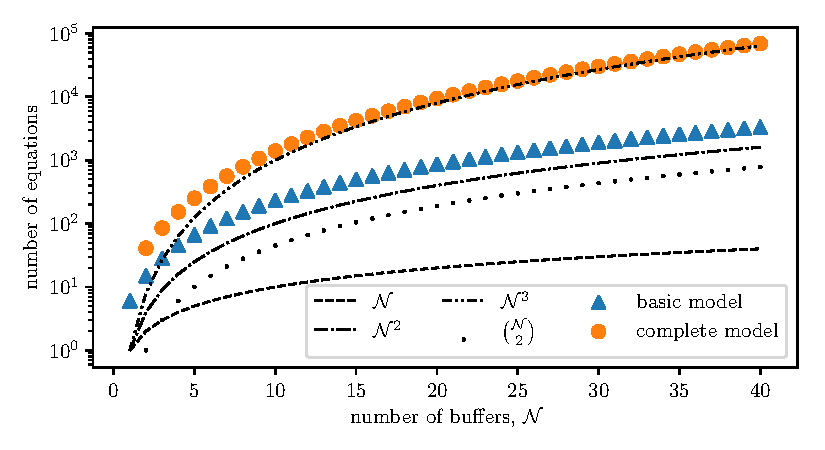
\includegraphics[angle=0,scale=0.55]{equations.pdf}
        \end{figure}
    \end{columns}
\end{frame}

\begin{frame}
    \frametitle{Results -- Random Example}
    Solving the random example yields the following result:
        \begin{table}
            \centering
            \caption{Required preparation vessels for random example}
            \begin{tabular}{r}
                vessel size\\ \hline
                \SI{2000}{\litre}\\
                \SI{8000}{\litre}\\
                \SI{25000}{\litre}\\
                \SI{30000}{\litre}\\
            \end{tabular}
        \end{table}
    Note that there may be many ways of assigning the buffers to these vessels
    and many feasible ways of scheduling these buffers.
    
    A feasible schedule may be represented graphically using an \emph{equipment
    time utilisation} plot.
\end{frame}

\begin{frame}
    \frametitle{Equipment Time Utilisation -- Random Example}
    \begin{figure}
        \centering
        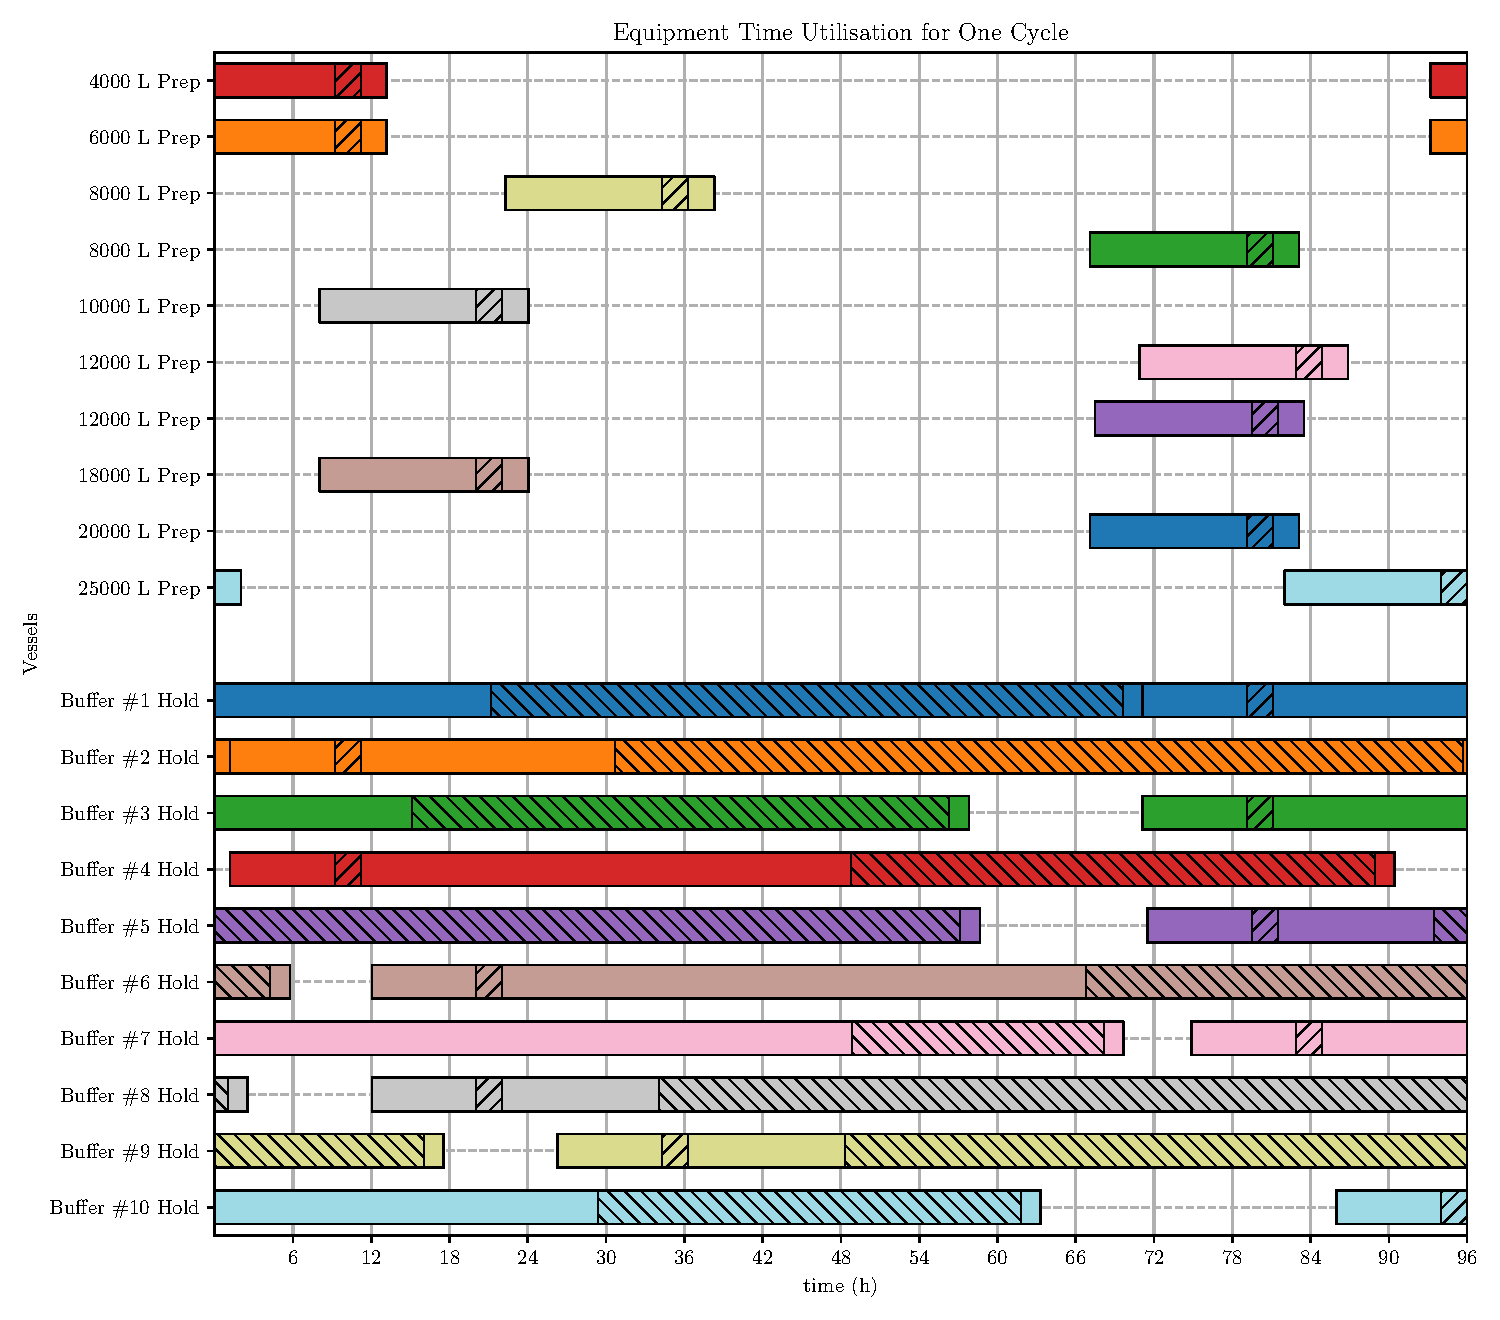
\includegraphics[angle=0,scale=0.55]{./../figures/plot1.pdf}
    \end{figure}
\end{frame}

\begin{frame}
    \frametitle{Goal Programming -- Reducing Hold Times}
    A \emph{better} feasible schedule may be obtained using \emph{goal
    programming}.
    
    The (original) objective function \underline{value} is fixed as a parameter
    and we replace the original objective function with a new one, which seeks to 
    minimise hold times.
    
    In doing so, hold times are minimised, but only to the extent that they
    don't interfere with the original list of required preparation vessels.
    \begin{figure}
        \centering
        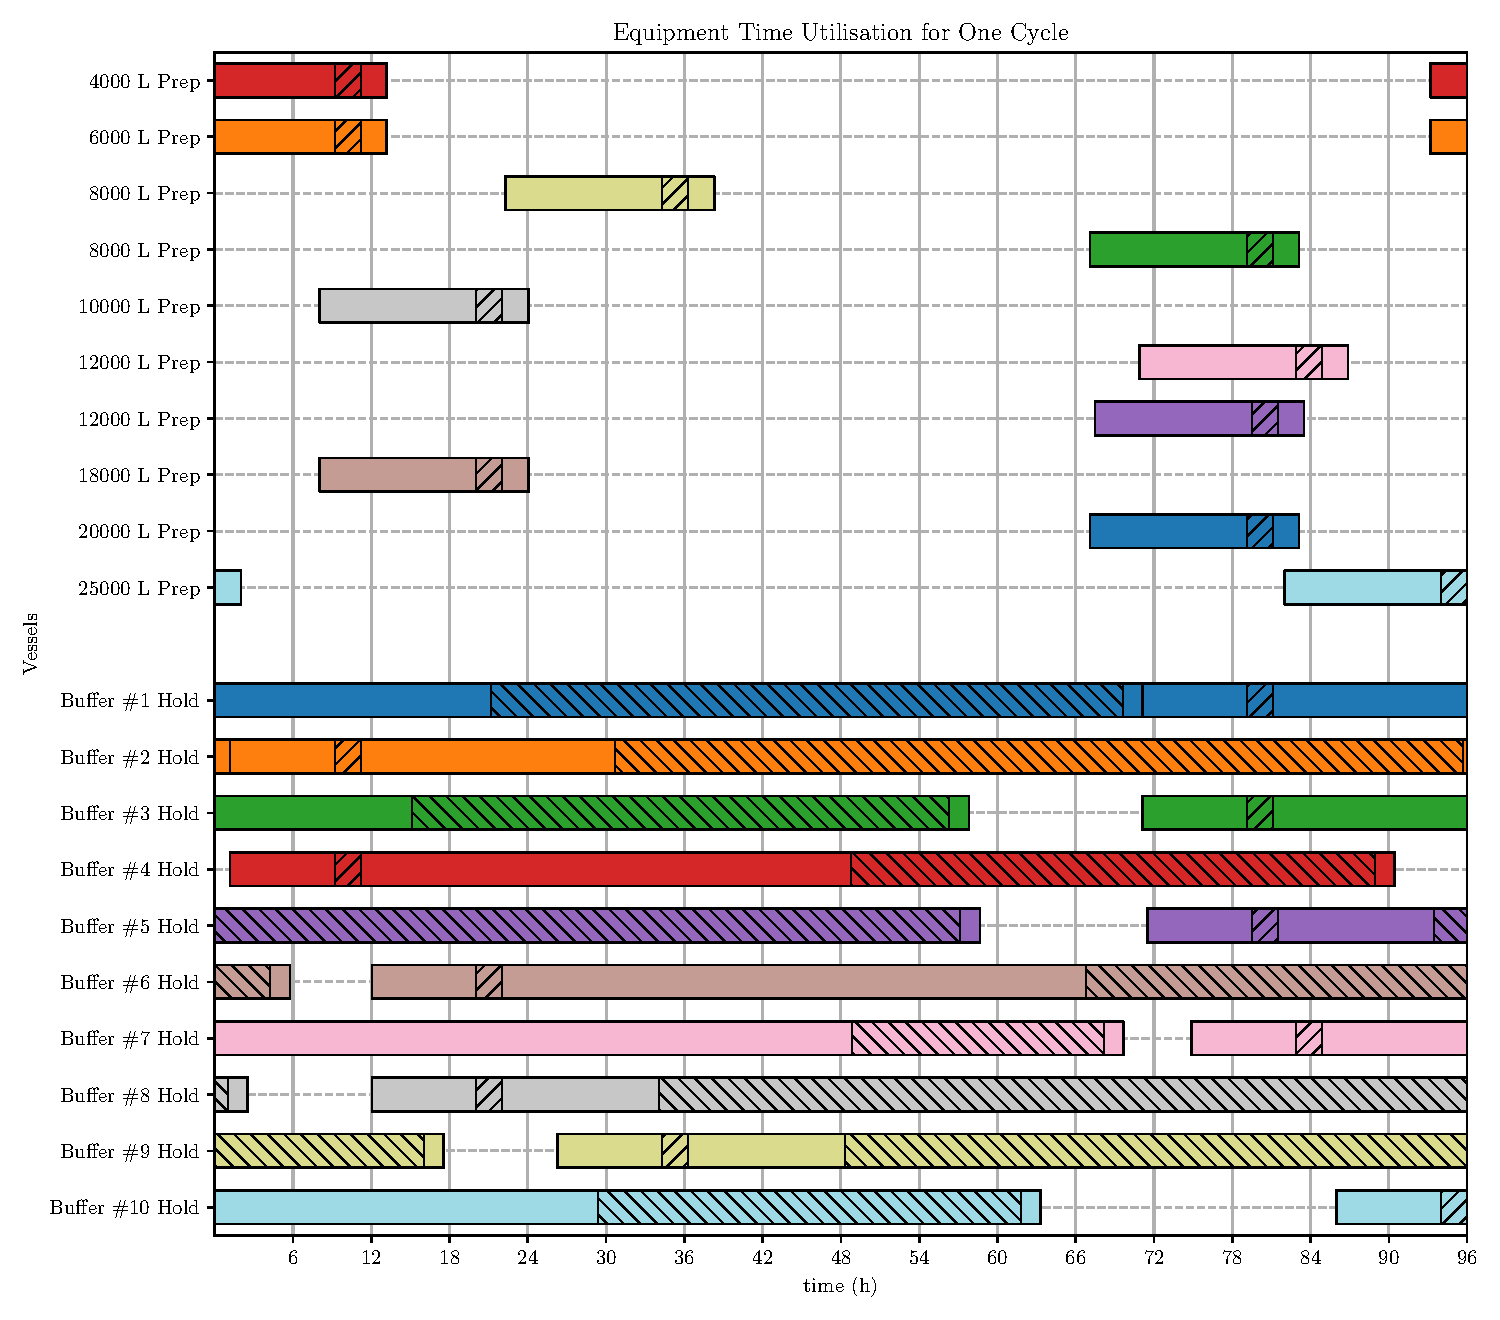
\includegraphics[width=0.495\textwidth]{./../figures/plot1.pdf}
        %\hfill
        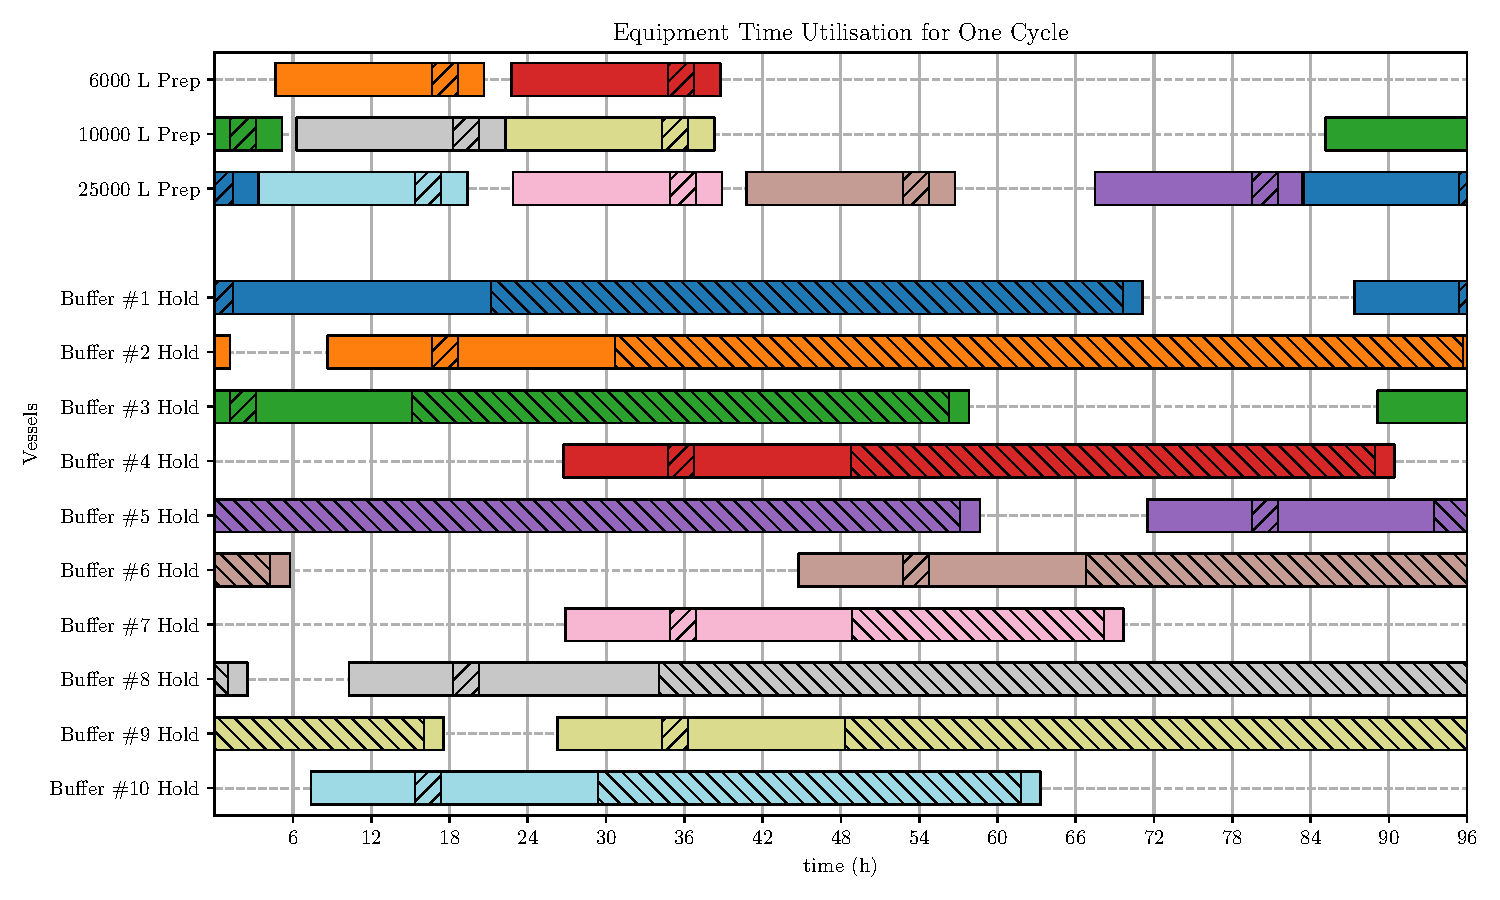
\includegraphics[width=0.495\textwidth]{./../figures/plot2.pdf}
    \end{figure}
\end{frame}

\begin{frame}
    \frametitle{Solution Time}
    \begin{figure}
        \centering
        \includegraphics[angle=0,scale=0.75]{timing.pdf}
    \end{figure}
\end{frame}

\begin{frame}
    \frametitle{Contribution}
    \begin{itemize}
        \item Academic
        \begin{itemize}
            \item No previous methodologies for solving such a problem could be
            found in the literature
            \item Contributes to the fields of process engineering and 
            linear programming
        \end{itemize}
        \vspace{1cm}
        \item Business
        \begin{itemize}
            \item Reduces time taken to generate early-stage designs
            \item Methodology ensures that a solution is provably optimum
            \item The ability to carry out the simulation and present visual
                results showcases expertise that differentiates a design firm's
                offering from its peers, helping to win further work.
        \end{itemize}
    \end{itemize}
\end{frame}

\begin{frame}
    \frametitle{Scope for Further Work}
    \begin{itemize}
        \item Add complexity to the model
        \begin{itemize}
            \item Material compatibility
            \item Non-dedicated hold vessels
            \item Multi-batch buffers
            \item Multi-product facilities
            \item Non-standard operations (e.g. buffers for chromatography
                column repacks)
        \end{itemize}
        \item Improve solution efficiency
        \begin{itemize}
            \item Specifying additional constraints may reduce search space
        \end{itemize}
        \item Further analysis of results
        \begin{itemize}
            \item Sensitivity analysis
            \item Monte-Carlo simulation
        \end{itemize}
    \end{itemize}
\end{frame}

\begin{frame}
    \begin{columns}
        \column{0.15\textwidth}
            \begin{figure}
                \centering
                
\includegraphics[angle=0,scale=0.03]{ucd_logo.png}
            \end{figure}
        \column{0.7\textwidth}
        \centering MSc in Business Analytics -- Dissertation\\
        \large \textbf{Optimising the design of buffer 
                       preparation in bioprocessing facilities}
        \column{0.15\textwidth}
            \begin{figure}
                \centering
                
\includegraphics[angle=0,scale=0.03]{ucd_logo.png}
            \end{figure}
    \end{columns}
    \centering \small \emph{Author: Sean Tully \quad Supervisor: Prof. Michael
        O'Neill}\par
    %\vspace{0.5cm}
    \begin{columns}
        \column{0.4\textwidth}
            \scriptsize \textbf{Aim}:
            \begin{itemize}
                \item  Development of a methodology and software tool
                for finding the optimum number, size and assignment of buffer
                preparation vessels in the design of a large-scale bioprocess
                facility
            \end{itemize}
            \textbf{Key Achievements}:
            \begin{itemize}
                \item Problem modelled as a MILP problem
                \item Code developed to solve problem
                \item Graphical representations generated of feasible
                    production schedules
                \item Goal programming carried out for further optimisation
            \end{itemize}
            
        \column{0.6\textwidth}
            \begin{figure}
                \centering
                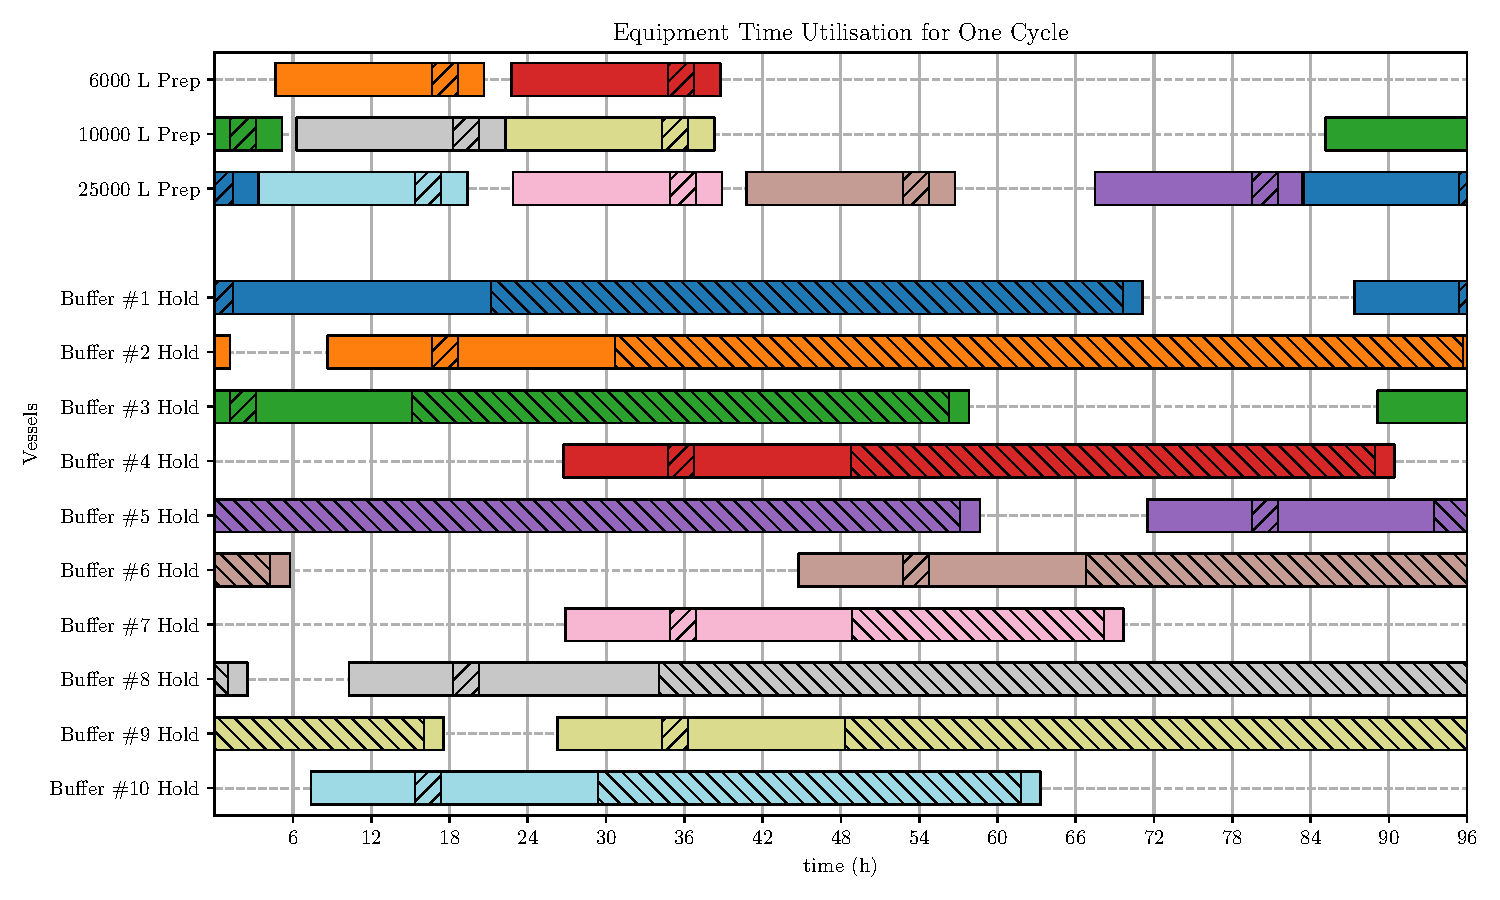
\includegraphics[width=0.9\textwidth]{./../figures/plot2.pdf}
                \captionsetup{justification=centering}
                \caption{\tiny Steady-State Equipment Time Utilisation plot
                showing a feasible schedule for a random problem with 12
                buffers, for a single cycle.}
            \end{figure}  
    \end{columns}
\end{frame}

\end{document}
